\documentclass[%
 aip,
% jmp,
% bmf,
% sd,
% rsi,
 amsmath,amssymb,
preprint,%
% reprint,%
%author-year,%
%author-numerical,
]{revtex4-2}

\usepackage{graphicx}
\usepackage{dcolumn}
\usepackage{bm}
%\linenumbers\relax % Commence numbering lines

\usepackage[utf8]{inputenc}
\usepackage[T1]{fontenc}
\usepackage{mathptmx}
\usepackage{etoolbox}
\usepackage{braket}
\usepackage{paralist}

%% Apr 2021: AIP requests that the corresponding 
%% email to be moved after the affiliations
\makeatletter
\def\@email#1#2{%
 \endgroup
 \patchcmd{\titleblock@produce}
  {\frontmatter@RRAPformat}
  {\frontmatter@RRAPformat{\produce@RRAP{*#1\href{mailto:#2}{#2}}}\frontmatter@RRAPformat}
  {}{}
}%
\makeatother

\newcommand\dstack[2]{\overset{#2}{#1}}

\renewcommand{\thetable}{S\arabic{table}}
\renewcommand{\thefigure}{S\arabic{figure}}
\renewcommand{\thepage}{S\arabic{page}}

\begin{document}


\title{Molecular responses in a snap: the \texttt{std2} package\\Supporting information}

\author{Pierre Beaujean}
 \affiliation{
Theoretical Chemistry Laboratory, Unit of Theoretical and Structural Physical Chemistry, Namur Institute of Structured Matter (NISM), University of Namur, Rue de Bruxelles, 61, B-5000 Namur (Belgium)
 }

\author{Marc de Wergifosse}
\email{marc.dewergifosse@uclouvain.be}
\affiliation{
	Theoretical Chemistry Group, Molecular Chemistry, Materials and Catalysis Division (MOST), Institute of Condensed Matter and Nanosciences, Université Catholique de Louvain, Louvain-la-Neuve B-1348 (Belgium)
}

\date{\today}
\maketitle

\begin{figure}[!h]
	\centering
	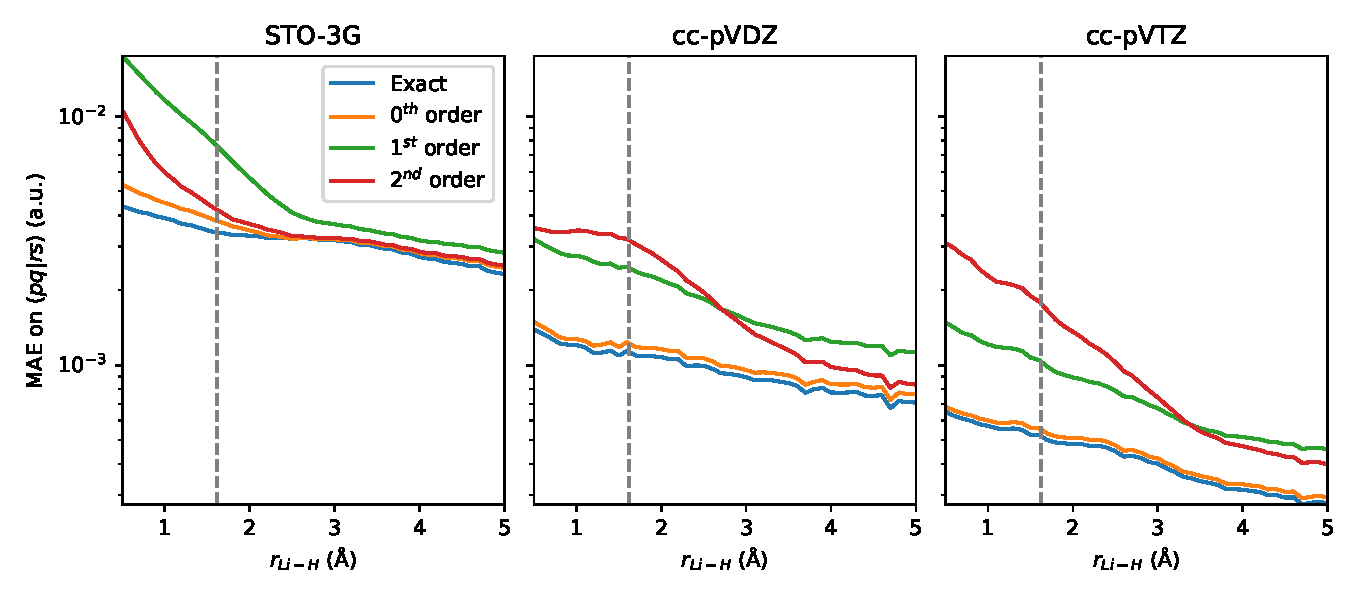
\includegraphics[width=\linewidth]{./FigureS1}
	\caption{Violin plots of the deviations in one-photon absorption (1PA) properties relative to RI-CC2 reference values for the QUEST dataset, as reported in Ref.~\citenum{maraldiEvaluatingPerformanceExact2025}, computed with the aug-cc-pVDZ basis set. Results are shown for several exchange--correlation functionals (XCFs) and levels of approximation (TD, sTD, and XsTD). Left: excitation energies. Right: oscillator strengths. For each method, the mean deviation is reported, with the MAD given in parentheses.}
\end{figure}


\begin{figure}[!h]
	\centering
	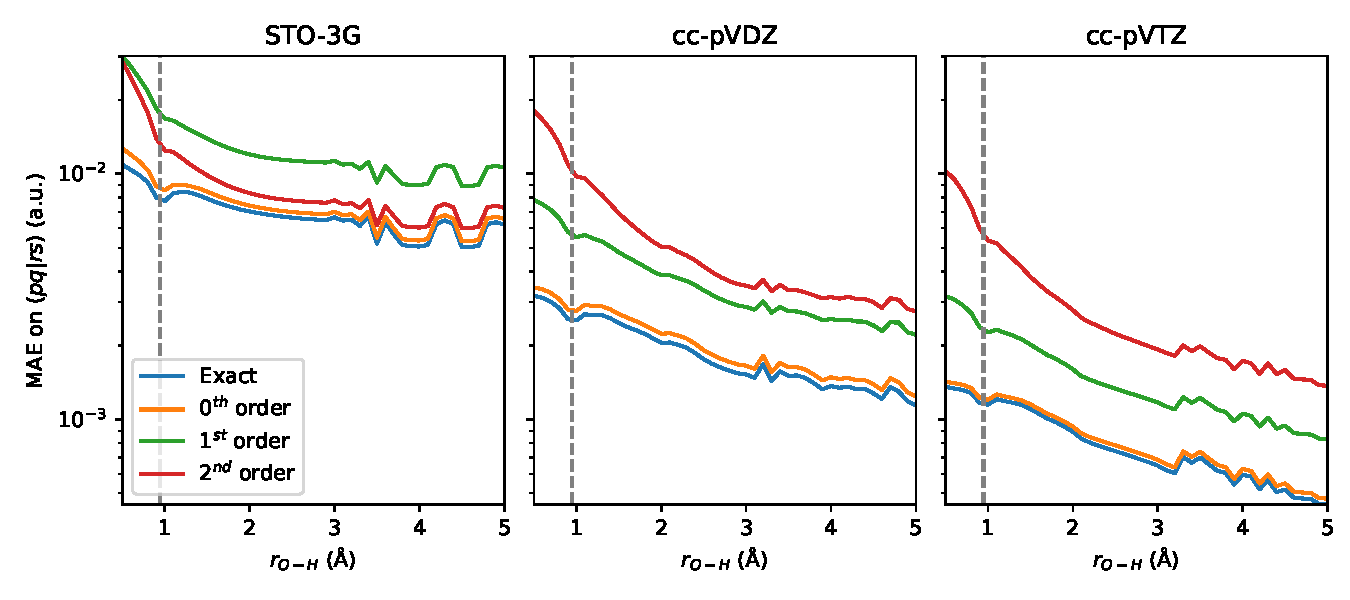
\includegraphics[width=\linewidth]{./FigureS2}
	\caption{Violin plots of the deviations in two-photon absorption (2PA) properties relative to RI-CC2 reference values for the QUEST dataset, as reported in Ref.~\citenum{maraldiEvaluatingPerformanceExact2025}, computed with the aug-cc-pVDZ basis set. Results are shown for several exchange--correlation functionals (XCFs) and levels of approximation (TD, sTD, and XsTD). Left: excitation energies. Right: 2PA strengths expressed as $\log_{10}(\delta^{\mathrm{2PA}})$. For each method, the mean deviation is reported, with the MAD given in parentheses.}
\end{figure}


\clearpage
\bibliography{biblio}

\end{document}
